\documentclass{beamer}
%
% Choose how your presentation looks.
%
% For more themes, color themes and font themes, see:
% http://deic.uab.es/~iblanes/beamer_gallery/index_by_theme.html
%
\mode<presentation>
{
  \usetheme{metropolis}   % or try Darmstadt, Madrid, Warsaw, ...
  \usecolortheme{default} % or try albatross, beaver, crane, ...
  \usefonttheme{default}  % or try serif, structurebold, ...
  \setbeamertemplate{navigation symbols}{}
  \setbeamertemplate{caption}[numbered]
} 

\usepackage[english]{babel}
\usepackage[utf8x]{inputenc}

% Code which makes the bracelet diagrams automatic
% The last two slides of this document show how to use this function
\usepackage{xifthen}                                                              % If statements in tex are trash
\usepackage{tikz}                                                                 % Allows us to draw diagrams
\directlua{dofile("bracelet.lua")}                                                % Import lua code
\newcommand{\bracelet}[2][]{
\ifthenelse{\isempty{#1}}{\directlua{bracelet(#2)}}{\directlua{bracelet(#2,#1)}}} % Bind latex to lua
% End of code which makes the diagrams automatic

% Code For Drawing Crosses
\newcommand{\cross}{
    	\draw[thick] (-1,3) -- ++(2,0)  --
        	      ++ (0,-2) -- ++(2,0)  --
                  ++ (0,-2) -- ++(-2,0) --
                  ++ (0,-2) -- ++(-2,0) --
                  ++ (0,2)  -- ++(-2,0) --
                  ++ (0,2)  -- ++(2,0)  -- ++(0,2);
}
\newcommand{\numberedcross}{
    	\draw[thick] (-1,3) -- node[fill=bg]{1} ++(2,0)  -- node[fill=bg]{2}
        	      ++ (0,-2) -- node[fill=bg]{3} ++(2,0)  -- node[fill=bg]{4}
                  ++ (0,-2) -- node[fill=bg]{5} ++(-2,0) -- node[fill=bg]{6}
                  ++ (0,-2) -- node[fill=bg]{7} ++(-2,0) -- node[fill=bg]{8}
                  ++ (0,2)  -- node[fill=bg]{9} ++(-2,0) -- node[fill=bg]{10}
                  ++ (0,2)  -- node[fill=bg]{11} ++(2,0) -- node[fill=bg]{12} ++(0,2);
}
% End of code for crosses

\title[Your Short Title]{Counting With Symmetries}
\author{Amber McKeough, Carlos Lira, Clarisse Bonnand, Ethan Kowalenko, Ethan Rooke, Reid Booth, Xavier Ramos}
\institute{UC Riverside}
\date{Date of Presentation}

\begin{document}

\begin{frame}
  \titlepage
\end{frame}

% Uncomment these lines for an automatically generated outline.
%\begin{frame}{Outline}
%  \tableofcontents
%\end{frame}

\section{Introduction}

\begin{frame}{Introduction - Reid}
\begin{columns}[T]
\begin{column}{.48\textwidth}
	\begin{center}
	\begin{tikzpicture}[scale=0.5, transform shape]
    	\bracelet{"white white white white white white"}
    \end{tikzpicture}
    \newline
    \begin{tikzpicture}
    	\draw (0,0) -- (5,0);
        \node[circle, fill=fg,inner sep=0pt,minimum size=.85cm] at (0,0) {};
    \end{tikzpicture}
    \end{center}
\end{column}%
\hfill%
\begin{column}{.48\textwidth}
	\begin{itemize}
		\item
        	We have black and white beads, and want to make
            a 6 bead bracelet.
        \item
        	Well, we have 6 beads and 2 choices per bead
            so $2^6$ right?
        \item
        	This is only true so long as you don't care about symmetry. 
	\end{itemize}
\end{column}%
\end{columns}
\end{frame}

\begin{frame}{Symmetry?}
	\begin{center}
	\begin{tikzpicture}[scale=0.5, transform shape]
    	\bracelet{"white black black black black black"}
        \begin{scope}[shift={(9cm,0)}]
        \bracelet{"black black black white black black"}
        \end{scope}
    \end{tikzpicture}
    \end{center}
    \begin{itemize}
    \item 
    	Our initial count considers these different
    \item
    	But one is just the other one rotated
    \item
    	We would like to consider these as the same when we count
    \end{itemize}
\end{frame}

\begin{frame}{The hard way}
	We can count this way by making a table of bracelets and counting how many different bracelets
    can be made via rotations of that bracelet.
\end{frame}
\begin{frame}{The hard way}
    \begin{columns}[T]
    \begin{column}{0.48\textwidth}
    \begin{tabular}{r l}
    	\raisebox{-.45\height}{\begin{tikzpicture}[scale=0.25, transform shape]
    		\bracelet{"white white white white white white"}
        	\begin{scope}[shift={(9,0)}]
        		\bracelet{"black black black black black black"}
        	\end{scope}
    	\end{tikzpicture}} & 2 \\
        
        \raisebox{-.45\height}{\begin{tikzpicture}[scale=0.25, transform shape]
    		\bracelet{"black white white white white white"}
        	\begin{scope}[shift={(9,0)}]
        		\bracelet{"white black black black black black"}
        	\end{scope}
    	\end{tikzpicture}} & 12 \\
        
        \raisebox{-.45\height}{\begin{tikzpicture}[scale=0.25, transform shape]
    		\bracelet{"black black white white white white"}
        	\begin{scope}[shift={(9,0)}]
        		\bracelet{"white white black black black black"}
        	\end{scope}
    	\end{tikzpicture}} & 12 \\
        
        \raisebox{-.45\height}{\begin{tikzpicture}[scale=0.25, transform shape]
    		\bracelet{"black white black white white white"}
        	\begin{scope}[shift={(9,0)}]
        		\bracelet{"white black white black black black"}
        	\end{scope}
    	\end{tikzpicture}} & 12
    \end{tabular}
    \end{column}%
	\hfill%
	\begin{column}{.48\textwidth}
        \begin{tabular}{r l}
    	\raisebox{-.45\height}{\begin{tikzpicture}[scale=0.25, transform shape]
    		\bracelet{"black white white black white white"}
        	\begin{scope}[shift={(9cm,0)}]
        		\bracelet{"white black black white black black"}
        	\end{scope}
    	\end{tikzpicture}} & 6 \\
        
        \raisebox{-.45\height}{\begin{tikzpicture}[scale=0.25, transform shape]
    		\bracelet{"black black white black white white"}
        	\begin{scope}[shift={(9cm,0)}]
        		\bracelet{"white white black white black black"}
        	\end{scope}
    	\end{tikzpicture}} & 12 \\
        
        \raisebox{-.45\height}{\begin{tikzpicture}[scale=0.25, transform shape]
    		\bracelet{"black black black white white white"}
    	\end{tikzpicture}} & 6 \\
        
        \raisebox{-.45\height}{\begin{tikzpicture}[scale=0.25, transform shape]
    		\bracelet{"black white black white black white"}
    	\end{tikzpicture}} & 2 

        \end{tabular}
    \end{column}
    \end{columns}
\end{frame}

\begin{frame}{The Goal}
	
    The goal of this talk is to develop a framework for 
    answering coloring questions like these where symmetry
    is crucial
\end{frame}

\section{Polya Build up - Ethan} 

\begin{frame}{Permutations}
	\begin{itemize}
	\item A permutation is a bijection from a set S into it's self
    \item Can be viewed as changing the order of elements
    \item Consider the set $S = \{1,2,3,4\}$ And let $f : S \to S$ be defined
    \begin{align*}
    	f(1) &= 2 \\
        f(2) &= 1 \\
        f(3) &= 4 \\
        f(4) &= 3 \\
    \end{align*}
	\end{itemize}
\end{frame}

\begin{frame}{Permutations}
	\begin{itemize}
	\item To specify permutations we use the following notation
    	\begin{itemize}
    	\item $(12)(34)$ 
    	\item $(13)(2)(4)$
    	\item $(1)(2)(3)(4) = e$
    	\end{itemize}
    \item From this notation it is pretty straight forward to find the composition of 
    	  two permutations. 
          \only<1>{\[(1234)(13)(24)=\phantom{(1432)}\]}
          \only<2>{\[(1234)(13)(24)=(14\phantom{32)}\]}
          \only<3>{\[(1234)(13)(24)=(143\phantom{2)}\]}
          \only<4>{\[(1234)(13)(24)=(1432)\]}
    \item The set of all permutation on sets of $n$ elements is $S_n$
	\end{itemize}
\end{frame}

\begin{frame}{Symmetry}
	This gives us a language to discuss symmetry now. Consider the two bracelet from earlier:
	\begin{center}
    	\begin{tikzpicture}[scale=0.5, transform shape]
    		\bracelet[true]{"white black black black black black"}
        	\uncover<2>{
            \draw[|->, thick] (3.75,0) -- (8.25,0);
        	\node[above] at (6,0.1) {\huge (14)(25)(36)};}
        	\begin{scope}[shift={(12,0)}]
        	\bracelet[true]{"black black black white black black"}
        	\end{scope}
    	\end{tikzpicture}
    \end{center}
\end{frame}

\begin{frame}{Symmetry}
	Thus we can describe the symmetry of an object by defining a subset of permutations
    we allow on it. We require that for any two permutations in our subset that their
    composition must also be in our set and that that every permutations inverse is
    in our set. 
    
    Taking our bracelet example from earlier we see that our set of permutations is:
    \[\{e,(123456),(135)(246),(14)(25)(36),(153)(264),(165432)\}\]
\end{frame}

\section{How to use Polya - Carlos}

\begin{frame}{Invariant Set $C_{\pi}$}
\begin{itemize}
\item Given a set of objects S, A set of colorings C (i.e. functions assigning colors to these objects) and a group G, we can denote the set of colors not changing when acted upon any permutation ${\pi}$ in G, as $C_{\pi}$.
\item For example, given a permutation (12)(3456) in G and letting w = white and b = black, a possible coloring in $C_{\pi}$ would be $c =(bbwwww)$ because the coloring remains unchanged under the permutation. Yet, a coloring (bwwwww) would not belong in the invariant set because the permutation would cause the color b to become w and the w in the first position to become b.
\end{itemize}
\end{frame}
%
%
\begin{frame}{Burnsides Lemma}
\begin{itemize}
\item Let the number N correspond to the number of equivalence classes of the set of colorings C. Each equivalence class is formed by an equivalence relaion ~, where two colorings in C are related if one coloring can be  transformed to the other via a permutation in G.
\item For example, let a permutation in G be defined by $(165432)$. Then, this permutation will simply rotate any coloring, meaning that the initial coloring and the coloring after the permutation acts on, will be the same.
\item Therefore we define Burnsides Lemma: $N=\frac{1}{\vert G\vert}{\displaystyle \sum_{n\in G}\vert C_{\pi}\vert}$
\end{itemize}
\end{frame}
%
%
\begin{frame}{Burnsides Lemma}
\begin{itemize}
\item The problem of using Burnsides Lemma is that the size of the invariant set $\vert C_{\pi}\vert$ must be computed with any permutation, $\pi$ , in the group G
\item A better way is to observe that a coloring invariant under the action of a permutation in G, implies that every object permuted by one cycle of $\pi$ must have the same color
\end{itemize}
\end{frame}
%
%
\begin{frame}{Cycle Index}
\begin{itemize}
\item As a generalization if $\pi$ has k disjoint cycles, then $\vert C_{\pi}\vert$ equals $m^k$.
\item Therefore we obtain monomial $M_{\pi}(x_{1}, x_{2}, \ldots,x_{n}) = \displaystyle \prod_{i=1}^{k}x_{l_{i}}$ , where permutation $\pi$ is a product of k disjoint cycles, each $x_{l_{i}}$ represents the length of each cycle, and the i'th cycle has length $l_{i}$.
\item For example, given $M_{(12)(34)}$ we obtain $x_{2}^{2}$.
\item Therefore we define the cycle index as $$P(x_{1}, x_{2}, \ldots,x_{n})=\frac{1}{|G|}\sum_{\pi\in G}M_{\pi}(x_{1}, x_{2}, \ldots,x_{n})$$.
\end{itemize}
\end{frame}

%
%
\begin{frame}{Polya}
\begin{itemize}
\item Let the set $\{y_{1}, y_{2}\}$ be a set of colors where $k_{i}$ is any color.
\item Using the group $\{(1)(2)(3)(4), (12)(34)\}$ and the cycle index $P(x_{1},x_{2}) = \frac{1}{2}(x_{1}^{4} + x_{2}^{2})$ we obtain the polynomial $P(y_{1}+y_{2} , y_{1}^{2}+y_{2}^{2}) = y_{1}^{4} + y_{2}^{4} + 2y_{1}^{3}y_{2} + 2y_{1}^{2}y_{2}^{3} + 4y_{1}^{2}y_{2}^{2}$.
\end{itemize}
\end{frame}

%
%
\begin{frame}{Polya}
\begin{itemize}
\item Choosing the term $4y_{1}^{2}y_{2}^{2}$ as an example and using the permutation (12)(34) we can see that the coefficient 4 represents four ways to color a set of object using the color $y_{1}$ twice for two objects in the permutation and $y_{2}$ twice for two objects in the permutation.
\end{itemize}
\end{frame}

\section{Using What We've Learned with an Example! - Amber}

\begin{frame}{An Application in Industry}

	%Consider the example:
    	Suppose a medical relief agency plans to design a symbol for their organization in the shape of a regular cross. To symbolize the purpose of the organization and emphasize its international constituency, its board of directors decides that the cross should be white in color, with each of the twelve line segments outlining the cross colored red, green, blue, or yellow, with an equal number of lines of each color.
%Based on the specifications of their design for their symbol, we'll be looking at the when 3 sides of the cross are colored red, 3 sides green, 3 sides blue, and 3 sides yellow.   
\end{frame}

\begin{frame}{An Application in Industry}
%However, as we now know, we have to consider the symmetries of the regular cross (rotations, flips that maintain the orientation of the polygon), so that we don't double-count essentially equivalent colorings.
	How many different ways are there to design the symbol, taking into account rotations and flips?
	\begin{center}
	\begin{tikzpicture}
    \cross
    \end{tikzpicture}
\end{center}
    
\end{frame}

\begin{frame}{An Application in Industry}
%To create the monomial for the regular cross, we'll consider the actions that will not alter the shape.
%(go to the board)
	%Identity
    %90deg rot
    %180deg rot
	First, WLOG we can number the sides of the cross as so:
    \begin{center}
	\begin{tikzpicture}
    \numberedcross
    \end{tikzpicture}
	\end{center}
\end{frame}

\begin{frame}{An Application in Industry}
The identity, the rotations...
\begin{itemize}
	\item Identity:
    	\begin{itemize}
    	\item cycle notation: $(1)(2)(3)(4)(5)(6)(7)(8)(9)(10)(11)(12)$
    	\item monomial: $x_1^{12}$
    	\item number of ways this occurs: $1$
    	\end{itemize}
    \item $90\deg$ rotation:
    	\begin{itemize}
    	\item cycle notation: $(1,4,7,10)(2,5,8,11)(3,6,9,12)$
    	\item monomial: $x_4^{3}$
    	\item number of ways this occurs: $2$
    	\end{itemize}
    \item $180\deg$ rotation:
    	\begin{itemize}
    	\item cycle notation: $(1,7)(2,8)(3,9)(4,10)(5,11)(6,12)$
    	\item monomial: $x_2^{6}$
    	\item number of ways this occurs: $1$
    	\end{itemize}
\end{itemize}
\end{frame}

\begin{frame}{An Application in Industry}
And the flips...
\begin{itemize}
\item Diagonal axis:
    	\begin{itemize}
    	\item cycle notation: $(1,10)(2,9)(3,8)(4,7)(5,6)(11,12)$
    	\item monomial: $x_2^{6}$
    	\item number of ways this occurs: $2$
    	\end{itemize}
\item Vertical/Horizontal axis:
    	\begin{itemize}
    	\item cycle notation: $(1,7)(2,6)(3,5)(4)(8,12)(9,11)(10)$
    	\item monomial: $x_1^{2} x_2^5$
    	\item number of ways this occurs: $2$
    	\end{itemize}
\end{itemize}
\end{frame}

\begin{frame}{An Application in Industry}
%We build the cycle index from the monomials we obtained from the symmetries with the coefficients being the number of ways that action can occur, and the outside coefficient being 1 over the size of the group of symmetries for this problem, which is also the total actions that can occur. (go back and count them? [quick])
From this, we get the cycle index:\\
%WRITE THIS ON THE BOARD:
\begin{center}
$P = \frac{1}{8}(x_1^{12}+2x_4^3 +3x_2^6 +2x_1^2 x_2^5)$
\end{center}
We want the coefficient of $r^3g^3b^3y^3$, so we look at\\ 
$x_1^{12}$, $x_4^{3}$, $x_2^{6}$, $x_1^{2} x_2^5$ individually.\\
(where $r$ = red, $g$ = green, $b$ = blue, $y$ = yellow)
\end{frame}

\begin{frame}{An Application in Industry}
Using Pólya's Enumeration Theorem, plugging in the colors $r,g,b,y$:\\
\begin{align*}
x_1 &= r+g+b+y\\
x_2 &=r^2+g^2+b^2+y^2\\
x_4 &=r^4+g^4+b^4+y^4\\
\end{align*}
So looking at each term individually:
\begin{align*}
x_1^{12} &= (r+g+b+y)^{12}\\
x_4^3 &=(r^4+g^4+b^4+y^4)^3\\
x_2^6 &=(r^2+g^2+b^2+y^2)^6\\
x_1^{2}x_2^5 &= (r+g+b+y)^2(r^2+g^2+b^2+y^2)^5\\
\end{align*}
%x_4^3 term will not give any r^3b^3g^3y^3 term because only even powers
%also none b/c (r^2+g^2+b^2+y^2)^5 has all terms with at least one power \ge 4
%eg. r^2g^2b^2y^2r^2 = r^4g^2b^2y^2
%we're looking for the coefficient of $r^3g^3b^3y^3$
\end{frame}

\begin{frame}{An Application in Industry}
\begin{itemize}
\item $P = \frac{1}{8}(x_1^{12}+2x_4^3 +3x_2^6 +2x_1^2 x_2^5)$
\end{itemize}
So the ways to get the coefficient for $r^3g^3b^3y^3$ from $P$ are...\\ 
\begin{align*}
&\frac{1}{8}{{12}\choose{3,3,3,3}}+\frac{1}{4}(0) + \frac{3}{8}(0) + \frac{1}{4}(0)
\end{align*}
$=46200$\\
\vspace{40pt}
Therefore, we have found that there are 46,200 different ways to design the symbol.
\end{frame}

\begin{frame}{An Interesting Find}
\begin{itemize}
\item While working on this example, we discovered that the group of symmetries for the edges of a regular cross is actually the dihedral group $D_4$, like that of a square.
%\item $D_4$ is the dihedral group for a regular polygon with 4 sides.
%\item The dihedral group $D_n$ is the group of symmetries for a regular polygon with $n$ sides, including reflections as well as rotations.
\item This is interesting! So we started looking into the effects of dihedral groups acting on polygons.
\end{itemize}
\end{frame}

%This slide is purely for notes that could be used in the dihedral group section:

%\begin{frame}{Dihedral Groups Acting on Polygons}
%Our findings:
%\begin{itemize}
%\item the action matters $\rightarrow$ how to embed/cut the polygon
%\item different ambient groups change things $\rightarrow$ not ambient under anything?
%\item $D_k$ formula for when k is prime
%\item what doesn't work: even k's because rotations get messed up due to subgroups of cyclic groups, ...?
%\end{itemize}
%paraphrasing; will elaborate further...
%\end{frame}

\section{Results, reflection groups, pictures - Clarisse}	
\begin{frame}{Group Action}
For the purposes of analyzing $D_k$ dihedral groups acting on $nk-gons$, it is best to imagine the $nk-gon$ inscribed inside the $k-gon$, and being restricted to the rotations and flips of the $k-gon$.\\
\end{frame}

\begin{frame}{Algorithm for constructing the polynomials  which represent a dihedral group $D_k$ acting on a $nk-gon$.}
	\begin{itemize}
    	\item construct the normal k-gon.
        	\begin{itemize}
            	\item Rotations
                \item Flips
             \end{itemize}
        \item Account for the n-cases
    \end{itemize}
\end{frame}

\begin{frame}{Rotations}
    First approach the normal k-gon. In order to construct the terms which represent rotations of the normal $k-gon$ we will take the following steps:\\
\end{frame}
\begin{frame}
	\begin{itemize}
		\item	Suppose $a_1,a_2,...,a_n$ are divisors of $k$.\\
 		\item For each divisor $a_i$ assemble the values which are coprime to it. \\
		\item Denote these coprime values $b_{ij}$ for each respective $a_i$.\\
		\item Now the \textbf{rotation} terms in our polynomial for the normal $k-gon$ will be:\\
		\begin{center}
        $\sum |b_{ij}|x^{k/a_i}_{a_i}$
        \end{center}
	\end{itemize}
\end{frame}
\begin{frame}{}
So 
\begin{center}
        $\sum |b_{ij}|x^{nk/a_i}_{a_i}$
        \end{center}
\end{frame}

\begin{frame}{Flips}
 Next, in order to find the polynomial of $d_k \circlearrowright nk-gon$ we need to add in the terms which represent flips.\\
	If $k$ is prime, then we have three cases:
			\begin{enumerate}
				\item $ kx_1^1x_2^{(kn-1)/2}$  for n odd $\longmapsto$\\
				\item $kx_2^{(kn)/2}$ for n even$\longleftrightarrow$\\
                \item $kx_1^2 x_2^{(kn-2)/2}$ for n even $|--|$\\
			\end{enumerate}
		  
\end{frame}

\begin{frame}{Understanding the Different Cases Concerning Flips}
%\includegraphics[width=\textwidth]{your-figure's-file-name}

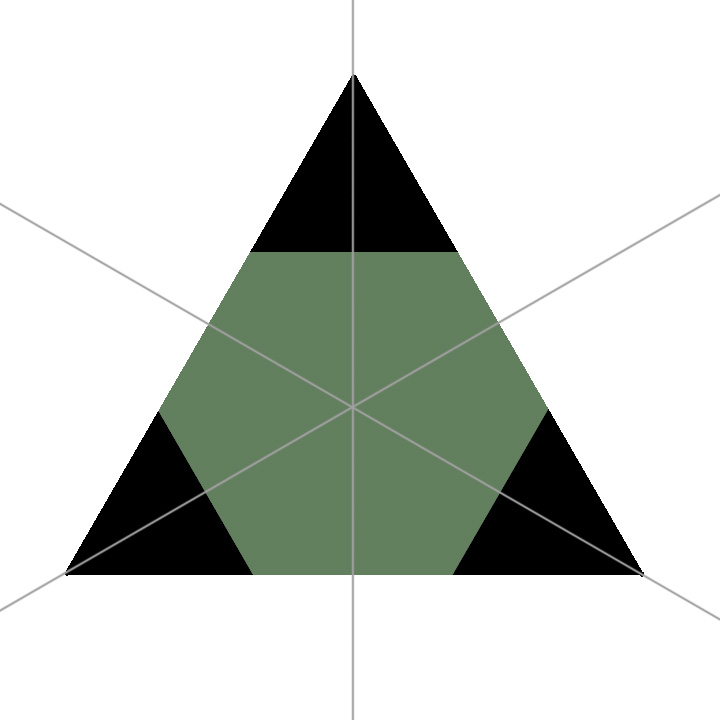
\includegraphics[width=3cm]{newtriangle_copya.jpg}
$x_1^6+2x_3^2+3x_1^2x_2^2$\\
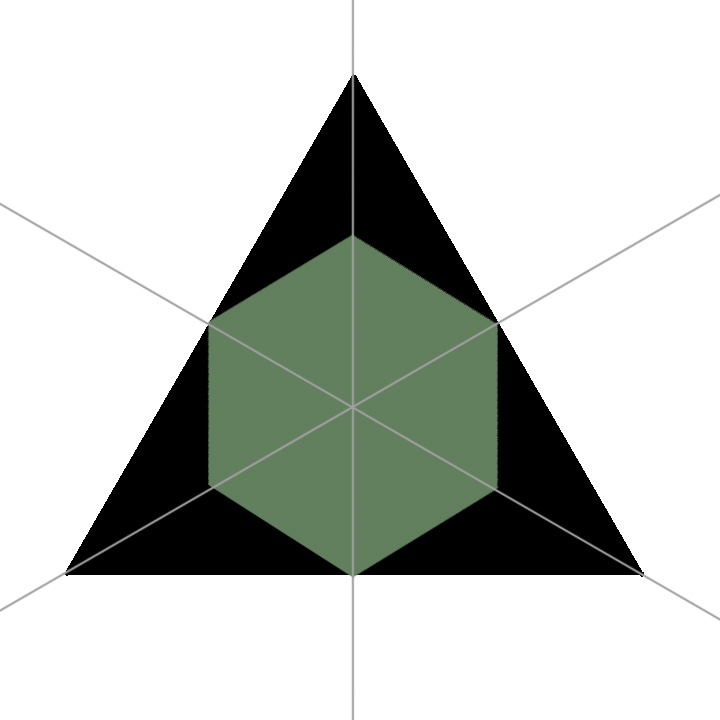
\includegraphics[width=3cm]{newtriangle_copy1.jpg}
$x_1^6+2x_3^2+ 3x_2^3$\\
\end{frame}

\begin{frame}
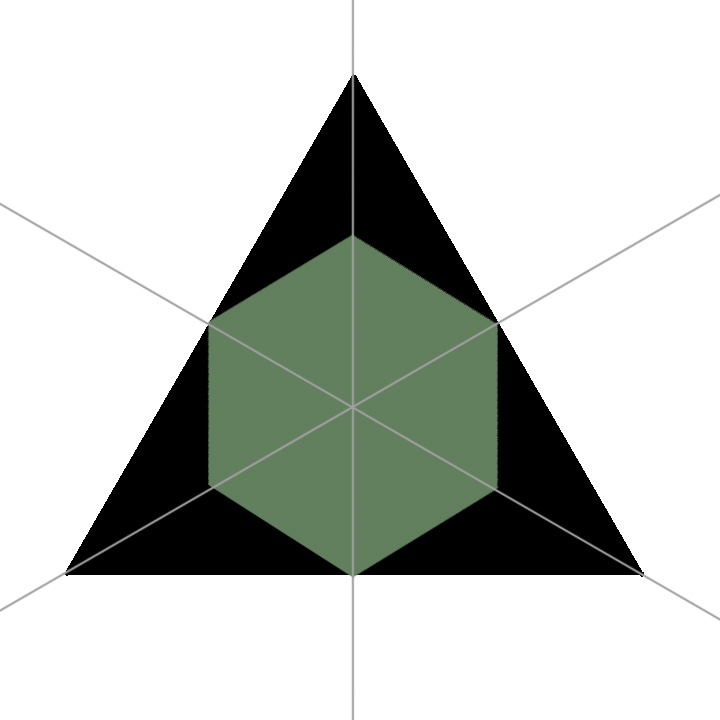
\includegraphics[width=3cm]{newtriangle_copy1.jpg}
\mapsto
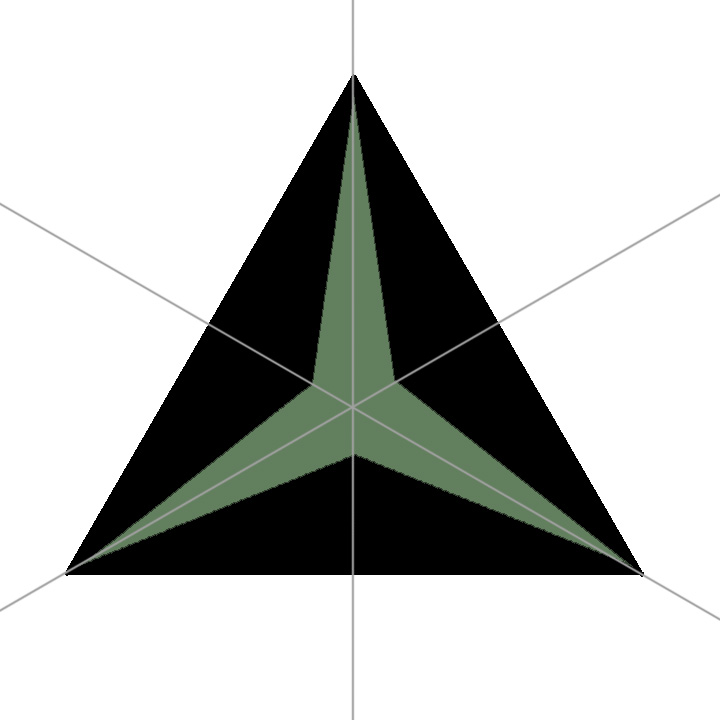
\includegraphics[width=3cm]{newtriangle_copyb.jpg}
\end{frame}

\begin{frame}
Cycle index of a triangle:
$x_1^3+2x_3^1+3x_1^1 x_2^1$\\

\begin{table}
\centering 
\begin{tabular}{l|c|l}
n & Truncated Vertices & Subdivision of Edges\\ \hline
2 & $x_1^6+2x_3^2$+\colorbox{yellow}{$3x_1^2x_2^2$} & $x_1^6+2x_3^2$+ \colorbox{cyan}{$3x_2^3$}\\
3 & $x_1^9+2x_3^3$+\colorbox{pink}{$3x_1^1x_2^4$}  &  $x_1^9+2x_3^3$+\colorbox{pink}{$3x_1^1x_2^4$}\\
4 & $x_1^12+2x_3^4$+\colorbox{yellow}{$3x_1^2x_2^5$} & $x_1^12+2x_3^4$+\colorbox{cyan}{$3x_2^6$}\\
5& $x_1^15+2x_3^5$+\colorbox{pink}{$3x_1^1x_2^7$} & $x_1^15+2x_3^5$+\colorbox{pink}{$3x_1^1x_2^7$}\\
\end{tabular}
\caption{$D_3 \circlearrowright 3n-gon$}
\end{table}
\end{frame}

\begin{frame}
\begin{table}
\centering
\begin{tabular}{c|c|c}
n & Truncated Vertices & Subdivision of Edges\\\hline
2 &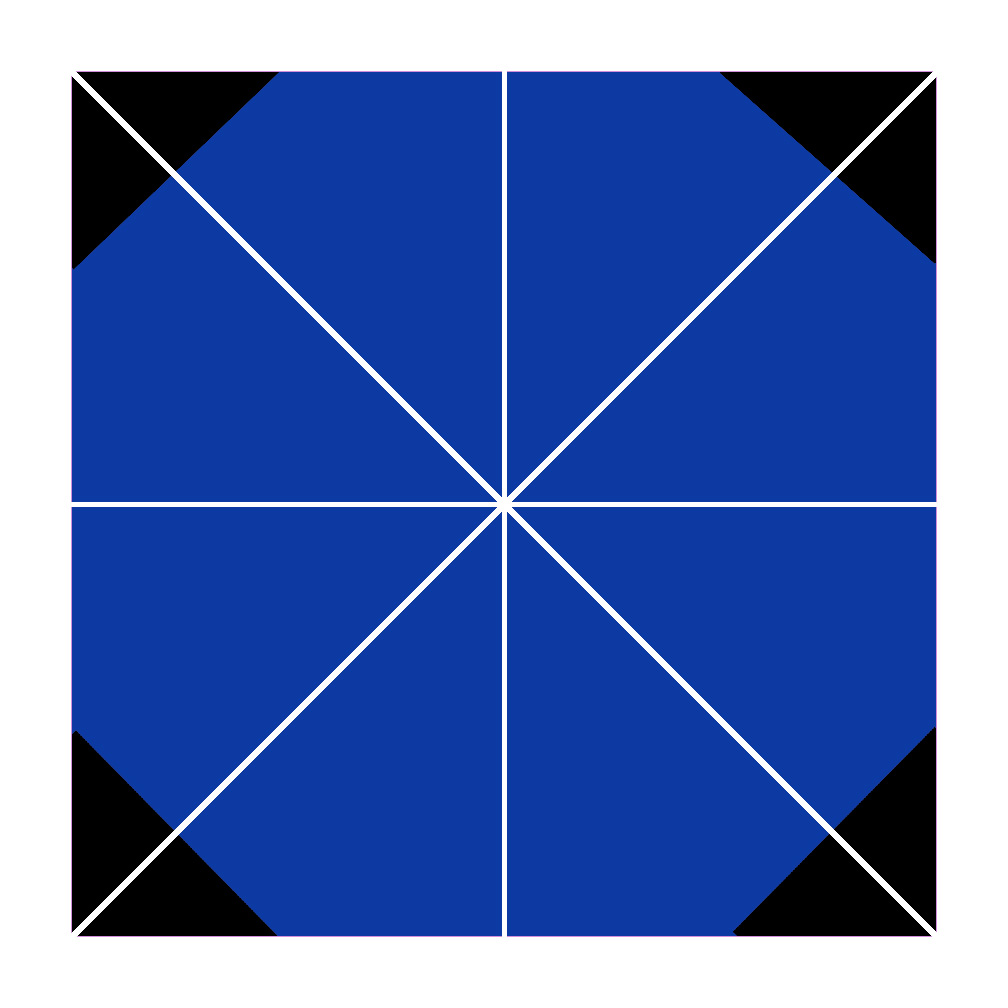
\includegraphics[width=3cm]{8tv}&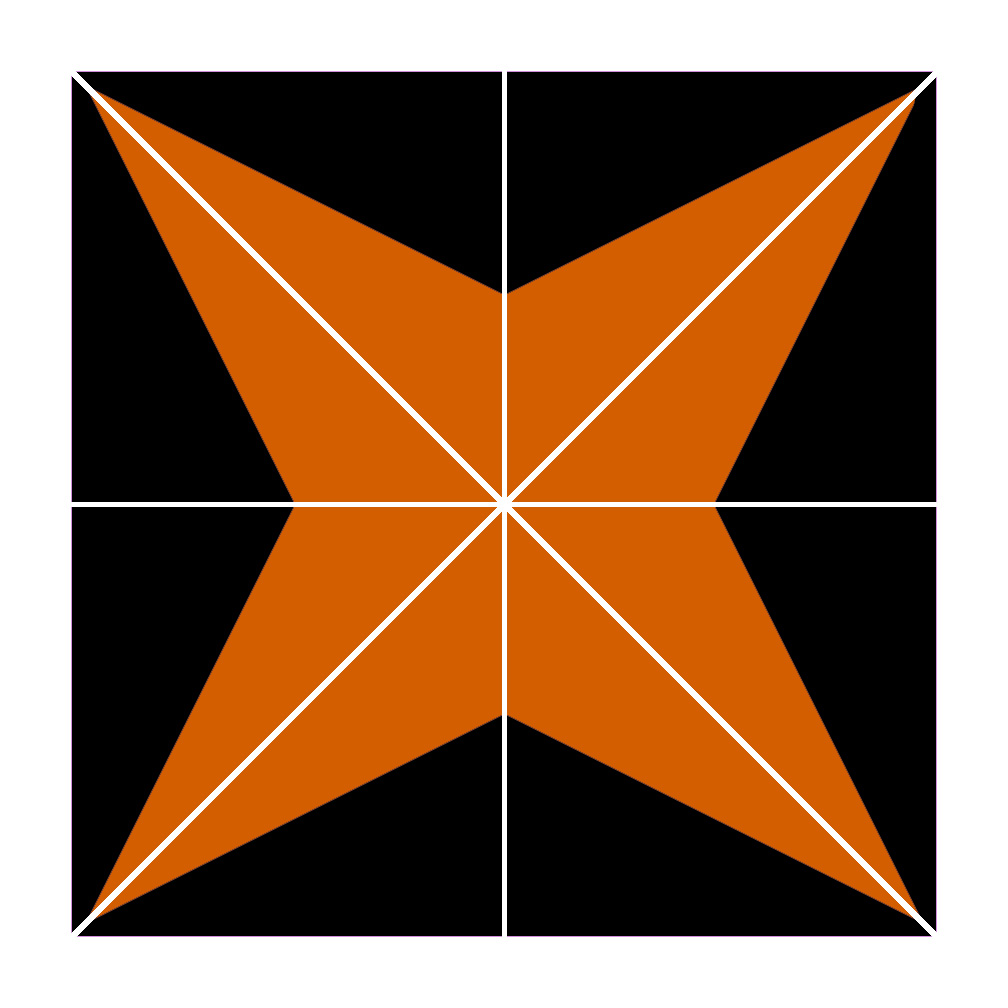
\includegraphics[width=3cm]{8se} \\\hline
3 & 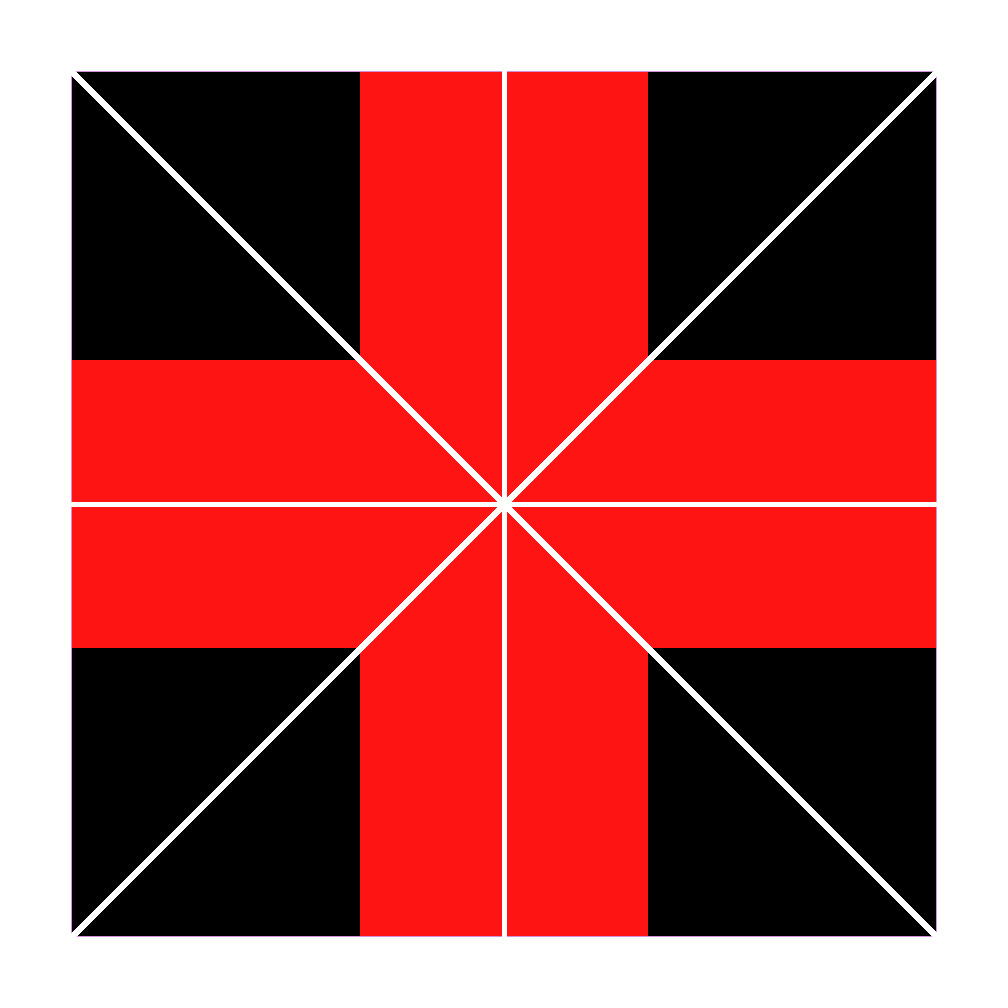
\includegraphics[width=3cm]{12tv} &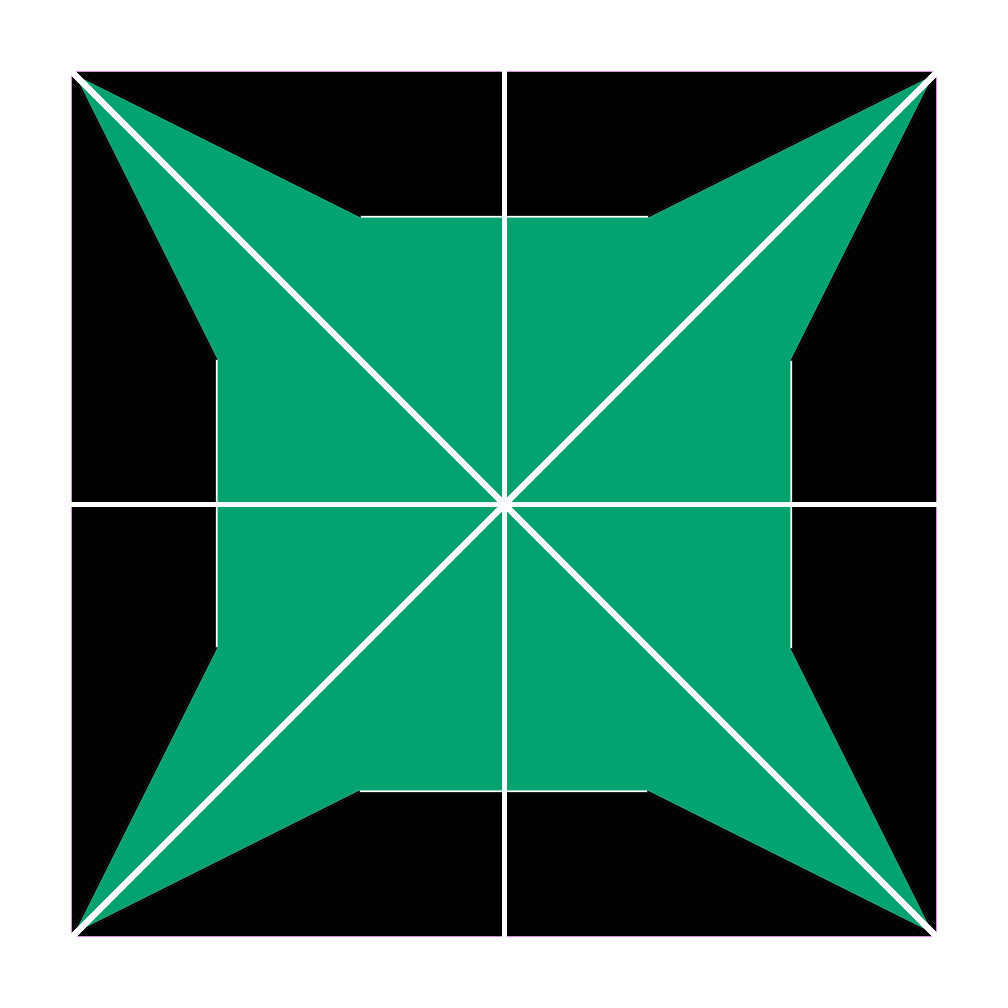
\includegraphics[width=3cm]{12se}\\\hline
\end{tabular}
\end{table}
\end{frame}

\begin{frame}
\begin{table}
\centering
\begin{tabular}{c|c|c}
n & Truncated Vertices & Subdivision of Edges \\\hline
5 & 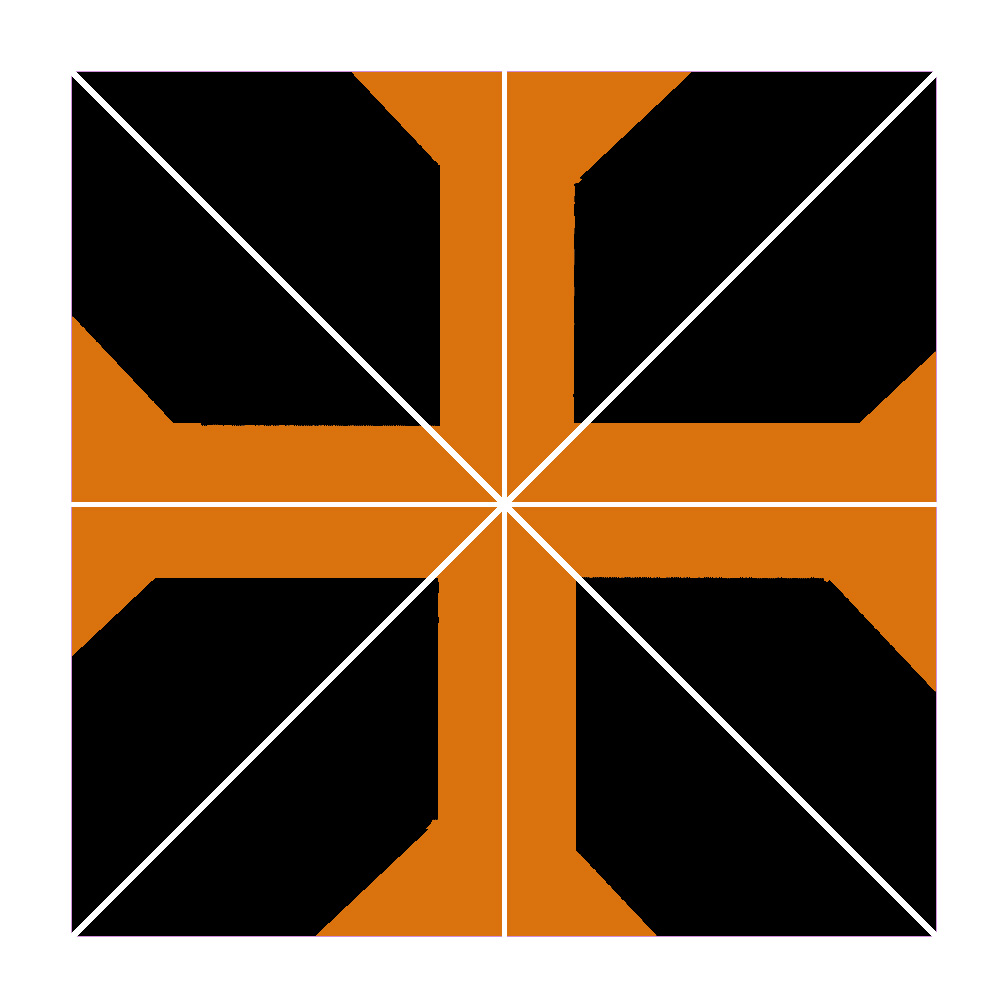
\includegraphics[width=3cm]{20tv} &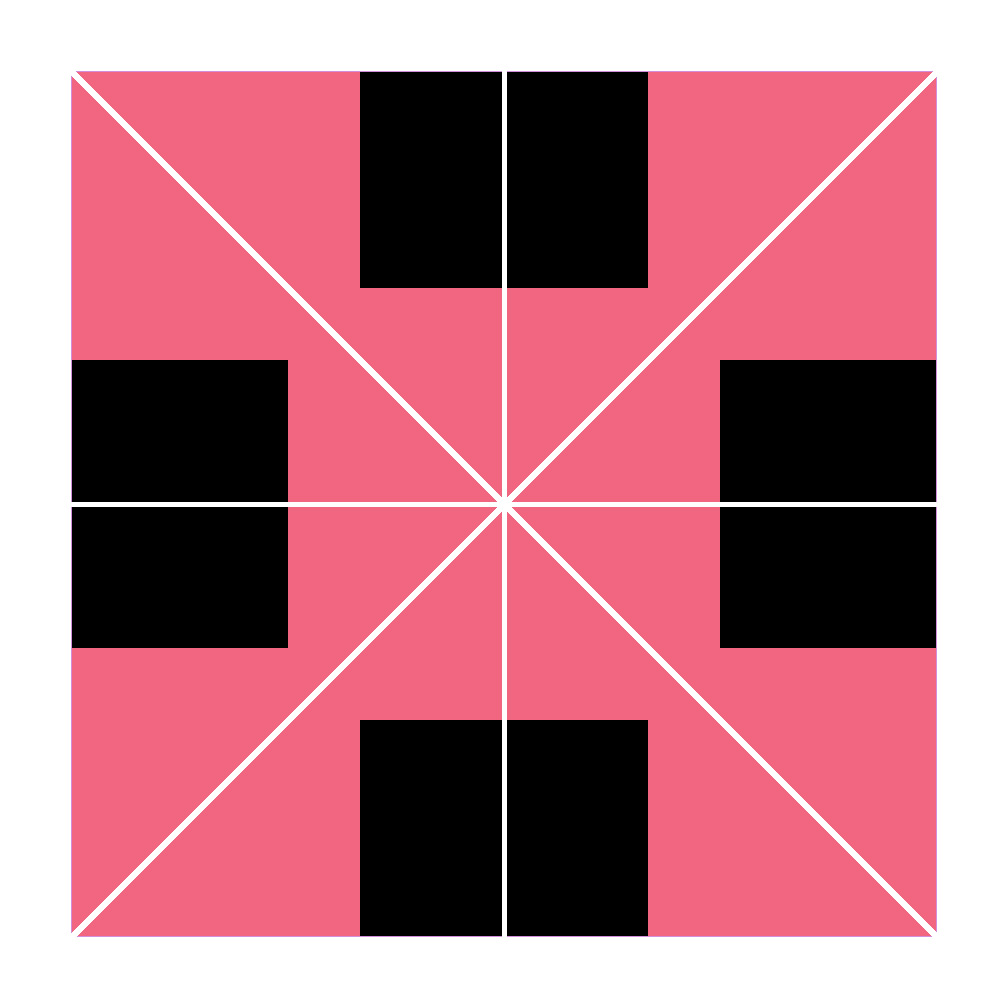
\includegraphics[width=3cm]{20se} \\\hline
6 &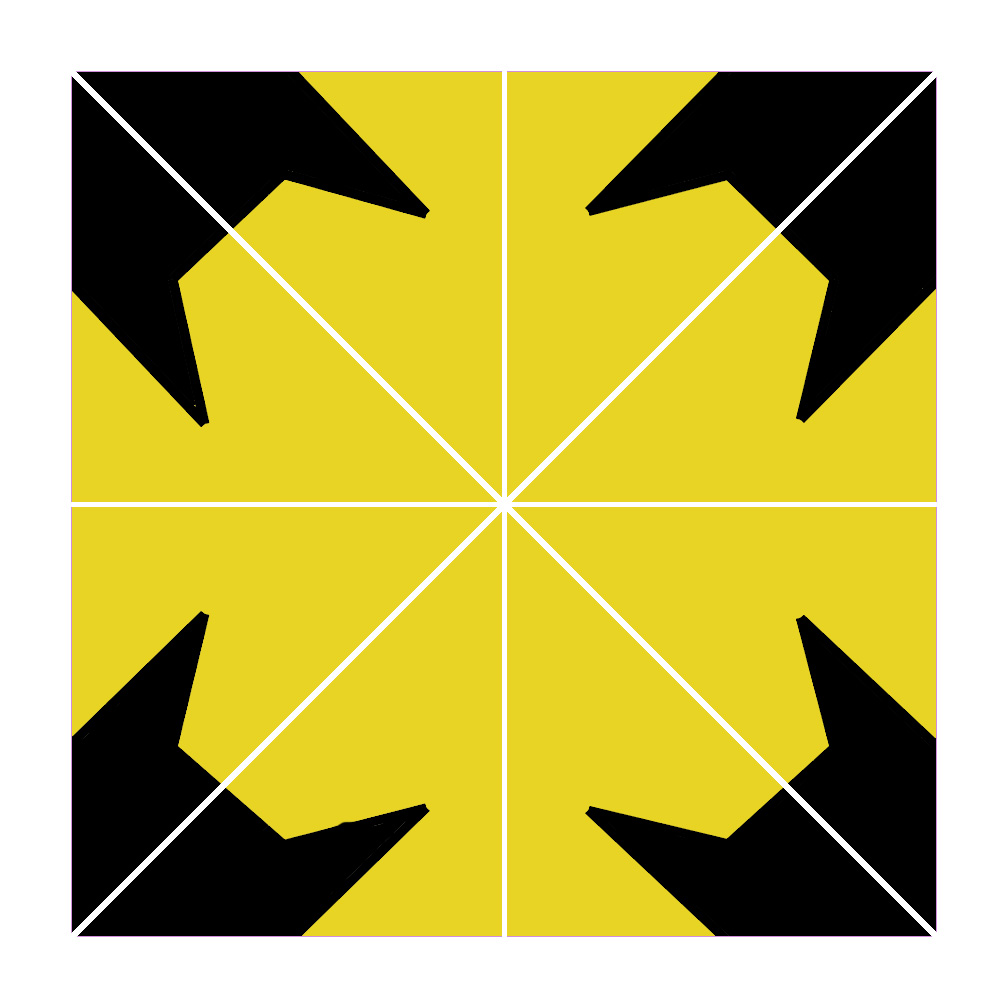
\includegraphics[width=3cm]{24_tv} &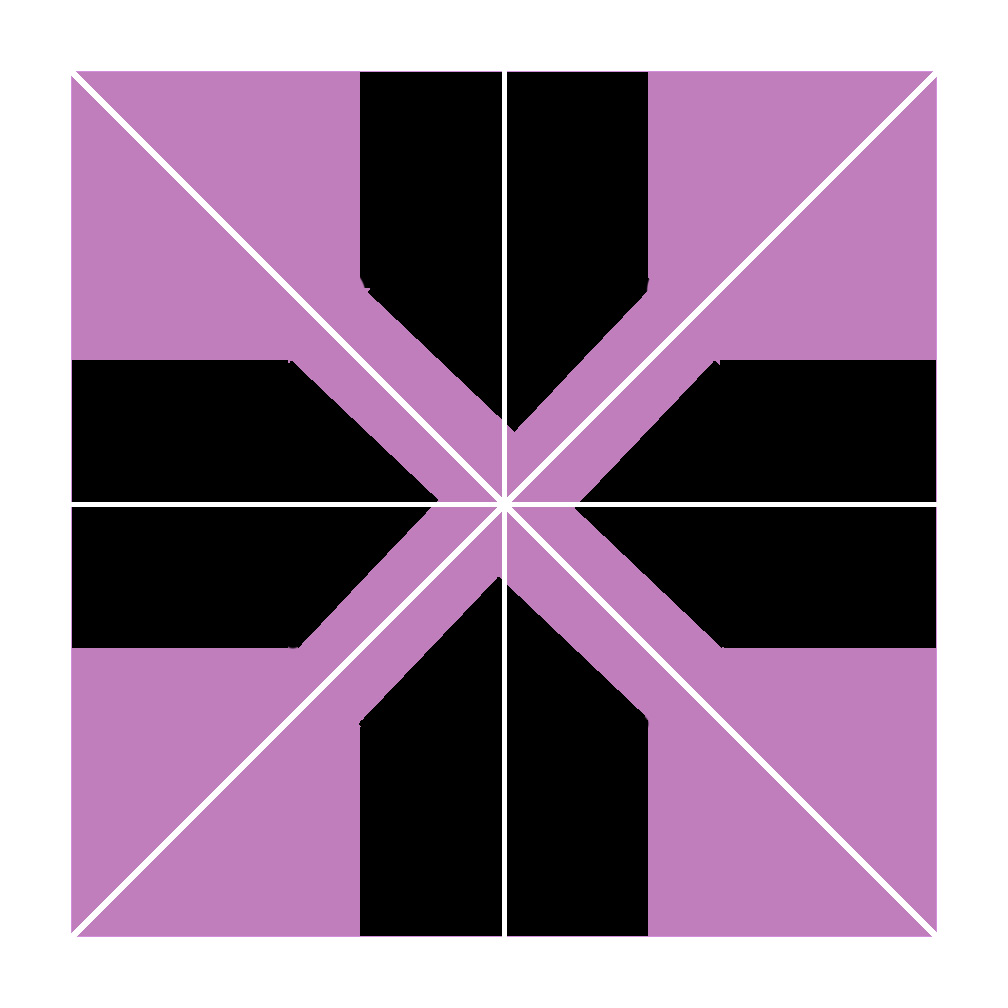
\includegraphics[width=3cm]{24se}\\\hline
\end{tabular}
\end{table}
\end{frame}

\begin{frame}
Cycle index of a square:
$x_1^4+2x_4^1+x_2^2+x_1^2x_2^1+2x_2^2$\\

$D_4 \circlearrowright 4n-gon$\\

\begin{table}
\centering 
\begin{tabular}{l|c|l}
n & Truncated Vertices & Subdivision of Edges\\ \hline
2 & 
$x_1^8+2x_4^2+x_2^4$+\colorbox{yellow}{$4x_1^2x_2^3$} &
$x_1^8+2x_4^2+x_2^4$+\colorbox{cyan}{$4x_2^4$}\\
3 &
$x_1^{12} +2x_4^3+x_2^6$+ \colorbox{yellow}{$2x_1^2x_2^5$}+\colorbox{cyan}{$2x_2^6$} &
$x_1^{12} +2x_4^3+x_2^6$+ \colorbox{yellow}{$2x_1^2x_2^5$}+\colorbox{cyan}{$2x_2^6$}\\
4 &
$x_1^{16}+2x_4^4+x_2^8$+\colorbox{yellow}{$4x_1^2x_2^7$} &
$x_1^{16}+2x_4^4+x_2^8$+\colorbox{cyan}{$4x_2^8$}\\
5 &
$x_1^{20}+2x_4^5+x_2^{10}$+\colorbox{yellow}{$2x_1^2x_2^4$}+\colorbox{cyan}{$2x_2^{10}$} & 
$x_1^{20}+2x_4^5+x_2^{10}$+\colorbox{yellow}{$2x_1^2x_2^4$}+\colorbox{cyan}{$2x_2^{10}$}\\
6 & $x_1^{24}+2x_4^6+x_2^{12}$+\colorbox{yellow}{$4x_1^2x_2^{11}$} & $ x_1^24+2x_4^6+x_2^{12}$+ \colorbox{cyan}{$4x_2^{12}$}\\

\end{tabular}
\caption{$D_4 \circlearrowright 4n-gon$}
\end{table}
\end{frame}

\begin{frame}{}
So for any $D_n$ acting on a $nk-gon$ we can produce the flips using cases:\\
	 $k$ Even:\\
			\begin{itemize}
    			\item $k/2x_1^2x_2^{(kn-2)/2}+k/2x_2^{kn/2}$ n odd ( $\longleftrightarrow$ and |--|)
                \item $kx_1^2x_2^{(kn-2)/2}$ n even (uniformly $|--|$)
                \item $kx_2^{kn/2}$ n odd (uniformly $\longleftrightarrow$ )
             \end{itemize}
         $k$ Odd:\\
         	\begin{itemize}
            	\item $kx_1^1x_2^{nk/2}$ n odd ($\mapsto$)
                \item $kx_2^{nk/2}$ n even ($|--|$)
                \item $kx_1^2x_2^{(nk-2)/2}$ n even ($\longleftrightarrow$)
            \end{itemize}

\end{frame}



\begin{frame}{3D Cases}

\end{frame}
\section{Some \LaTeX{} Examples}

\begin{frame}
	Past here are just examples of how to use code.  Should all be 
    removed before the presentation. 
\end{frame}

\subsection{Bracelets}

\begin{frame}{Drawing Bracelets Un-numbered}
	% To call the function you need to be in a tikz picture
    % To use the function you just feed it a string of space separated colors.
    % The first color starts at 12-o'clock and it moves clockwise.
    % Supported colors are: red, green, blue, cyan, magenta, yellow, black, darkgray
    % lightgray, brown, lime (please don't use lime), olive, orange, pink, purple, 
    % teal, violet, and white with the slight exception that black and white get 
    % replaced with the foreground and background color of our theme respectively. 
    % There are ways to define more, but cross that bridge if it ever comes
    % Example usage:
    \begin{center}
    	\begin{tikzpicture}
    		\bracelet{"red green blue cyan magenta yellow black gray darkgray lightgray"}
    	\end{tikzpicture}
    \end{center}  
\end{frame}
\begin{frame}{Drawing Bracelets Numbered}
    % To number the bracelet you just add a [true] before the {"color color color ..."} bit
    % Example Usage:
    \begin{center}
    	\begin{tikzpicture}
    		\bracelet[true]{"brown lime olive orange pink purple teal violet white"}
    	\end{tikzpicture}
    \end{center}
\end{frame}

\subsection{Cross}
\begin{frame}{Numbered}
\begin{center}
	\begin{tikzpicture}
    \numberedcross
    \end{tikzpicture}

\end{center}
\end{frame}

\begin{frame}{Un-numbered}
\begin{center}
	\begin{tikzpicture}
    \cross
    \end{tikzpicture}
\end{center}
\end{frame}

\subsection{Tables and Figures}

\begin{frame}{Tables and Figures}

\begin{itemize}
\item Use \texttt{tabular} for basic tables --- see Table~\ref{tab:widgets}, for example.
\item You can upload a figure (JPEG, PNG or PDF) using the files menu. 
\item To include it in your document, use the \texttt{includegraphics} command (see the comment below in the source code).
\end{itemize}

% Commands to include a figure:
%\begin{figure}
%\includegraphics[width=\textwidth]{your-figure's-file-name}
%\caption{\label{fig:your-figure}Caption goes here.}
%\end{figure}

\begin{table}
\centering
\begin{tabular}{l|r}
Item & Quantity \\\hline
Widgets & 42 \\
Gadgets & 13
\end{tabular}
\caption{\label{tab:widgets}An example table.}
\end{table}

\end{frame}

\subsection{Mathematics}

\begin{frame}{Readable Mathematics}

Let $X_1, X_2, \ldots, X_n$ be a sequence of independent and identically distributed random variables with $\text{E}[X_i] = \mu$ and $\text{Var}[X_i] = \sigma^2 < \infty$, and let
$$S_n = \frac{X_1 + X_2 + \cdots + X_n}{n}
      = \frac{1}{n}\sum_{i}^{n} X_i$$
denote their mean. Then as $n$ approaches infinity, the random variables $\sqrt{n}(S_n - \mu)$ converge in distribution to a normal $\mathcal{N}(0, \sigma^2)$.

\end{frame}
\end{document}
